\chapter{Troubleshooting}
\label{ch:troubleshooting}



\section{Walltime issues}
If you get from your job output an error message similar to this:

\begin{prompt}
 =>> PBS: job killed: walltime %\emph{<value in seconds>}% exceeded limit %\emph{<value in seconds>}%
\end{prompt}

This occurs when your job did not complete within the requested walltime.
See section~\ref{sec:specifying-walltime-requirements} for more information about how to request the walltime.
It is recommended to use \emph{checkpointing} if the job requires \strong{72 hours} of walltime or more to be executed.
% FIXME: Refer to Checkpointing section.



\section{Out of quota issues}

Sometimes a job hangs at some point or it stops writing in the disk. These errors are usually
related to the quota usage. You may have reached your quota limit at some storage endpoint.
You should move (or remove) the data to a different storage endpoint (or request more quota) to be able to write to the disk and then resubmit the jobs.
\ifgent
Another option is to request extra quota for your VO to the VO moderator/s.
See section~\ref{subsec:predefined-user-directories} and section~\ref{subsec:predfined-quotas} for more information about
quotas and how to use the storage endpoints in an efficient way.
\fi
% FIXME: Add how to request quota section

\section{Issues connecting to login node}
\label{sec:connecting-issues}

If you're confused about the SSH public/private key pair concept, maybe the
key/lock analogy in \autoref{subsec:how-do-ssh-keys-work} can help.

If you have errors that look like:

\begin{prompt}
%\userid{}%@%\loginnode%: Permission denied
\end{prompt}

or you are experiencing problems with connecting, here is a list of things to do
that should help:

\begin{enumerate}
    \item Keep in mind that it an take uup to an hour for your VSC account to become
        active after it has been \emph{approved}; until then, logging in to your VSC
        account will not work.
\ifmacORlinux
    \item Your SSH private key may not be in the default location (\verb|$HOME/.ssh/id_rsa|).
        There are several ways to deal with this (using one of these is sufficient):
\begin{enumerate}
            \item Use the \verb|ssh -i| (see section~\ref{sec:connect}) \emph{OR;}
            \item Use \verb|ssh-add| (see section~\ref{sec:using-ssh-agent-with-openssh}) \emph{OR;}
            \item Specify the location of the key in \verb|$HOME/.ssh/config|. You will
                need to replace the VSC login id in the \verb|User| field with your own:

            \begin{prompt}
Host %\hpcname%
    Hostname %\loginnode%
    IdentityFile %\emph{/path/to/private/key}%
    User %\emph{\userid}%\end{prompt}

    Now you can just connect with \texttt{ssh \hpcname}.
\end{enumerate}
\fi
        \item Please double/triple check your VSC login ID. It should look
            something like \emph{\userid}: the letters \verb|vsc|, followed
            by exactly 5 digits. Make sure it's the same one as the one on
            \url{https://account.vscentrum.be/}.
        \item You previously connected to the \hpc from another machine, but now
            have another machine? Please follow the procedure for adding additional
            keys in section~\ref{sec:adding-multiple-keys}. You may need to wait
            for 15-20 minutes until the SSH public key(s) you added become active.
        \item \ifwindows Make sure you're using the private key (not the public key) when trying to connect:
            If you followed the manual, the private key filename should end in
            \verb|.ppk| (not in \verb|.pub|).
            \else
            When using an SSH key in a non-default location, make sure you supply
            the path of the private key (and not the path of the public key)
            to \verb|ssh|. \verb|id_rsa.pub| is the usual filename of the public
            key, \verb|id_rsa| is the usual filename of the private key.
            (See also section~\ref{sec:connect})
            \fi
        \item If you have multiple private keys on your machine, please make sure
            you're using the one that corresponds to (one of) the public key(s) you
            added on \url{https://account.vscentrum.be/}.
        \item Please do not use someone else's private keys. You must never
            share your private key, they're called \emph{private} for a good reason.
\end{enumerate}

If you've tried all applicable items above and it doesn't solve your problem,
please contact \hpcinfo and include the following information:

\ifwindows
Please create a log file of your SSH session by following the steps
in \href{https://my.kualo.com/knowledgebase/?kbcat=0&article=888}{this article}
and include it in the email.
\else
Please add \verb|-vvv| as a flag to \verb|ssh| like:

\begin{prompt}
%\shellcmd{ssh -vvv \userid{}@\loginnode}%
\end{prompt}

and include the output of that command in the message.
\fi

\ifmacORlinux

\section{WARNING: REMOTE HOST IDENTIFICATION HAS CHANGED!}

If you get a warning that looks like the one below, it may be possible
that someone is trying to intercept the connection between you and the \hpc.

\begin{prompt}
@@@@@@@@@@@@@@@@@@@@@@@@@@@@@@@@@@@@@@@@@@@@@@@@@@@@@@@@@@@
@    WARNING: REMOTE HOST IDENTIFICATION HAS CHANGED!     @
@@@@@@@@@@@@@@@@@@@@@@@@@@@@@@@@@@@@@@@@@@@@@@@@@@@@@@@@@@@
IT IS POSSIBLE THAT SOMEONE IS DOING SOMETHING NASTY!
Someone could be eavesdropping on you right now (man-in-the-middle attack)!
It is also possible that a host key has just been changed.
The fingerprint for the ECDSA key sent by the remote host is
SHA256:1MNKFTfl1T9sm6tTWAo4sn7zyEfiWFLKbk/mlT+7S5s.
Please contact your system administrator.
Add correct host key in ~/.ssh/known_hosts to get rid of this message.
Offending ECDSA key in ~/.ssh/known_hosts:%\strong{21}%
ECDSA host key for %\loginnode{}% has changed and you have requested strict checking.
Host key verification failed.
\end{prompt}

You will need to remove the line it's complaining about (in the example, line 21).
To do that, open \verb|~/.ssh/config| in an editor, and remove the line. This
results in \verb|ssh| ``forgetting'' the \hpc.

After you've done that, you'll need to connect to the \hpc again.
See \autoref{sec:warning-message-new-host} to verify the fingerprints.
\strong{It's important to verify the fingerprints. If they don't match,
don't connect.}

\else

\section{WARNING - POTENTIAL SECURITY BREACH}

If you get a warning box that looks like the one below, it may be possible
that someone is trying to intercept the connection between you and the \hpc.
\strong{Do not click ``Yes'' or ``No'' until you verified the fingerprint}.

You will need to verify that the fingerprint show in the dialog matches one of the
following fingerprints:

\puttyFirstConnect

If it does, click ``Yes''.

If it doesn't (like in the example), take a screenshot, press ``Cancel'' and contact \hpcinfo.


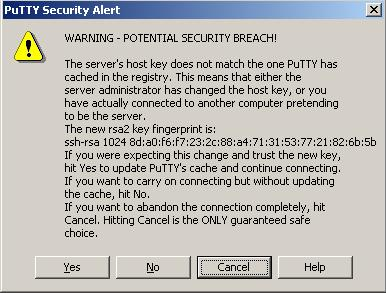
\includegraphics[width=0.5\textwidth]{putty_security_alert}


\fi


\section{DOS/Windows text format}

If you get errors like:

\begin{prompt}
%\shellcmd{qsub fibo.pbs}%
qsub:  script is written in DOS/Windows text format
\end{prompt}

It's probably because you transferred the files from a Windows computer.
Please go to the section about \verb|dos2unix| in \href{\LinuxManualURL#sec:dos2unix}{chapter 5 of the intro to Linux}
to fix this error.

\section{Warning message when first connecting to new host}
\label{sec:warning-message-new-host}

\ifmacORlinux
\begin{prompt}
%\shellcmd{ssh \userid{}@\loginnode{}}%
The authenticity of host %\loginnode% (<IP-adress>)
can't be established.
%\underline{<algorithm> key fingerprint is <hash>}%
Are you sure you want to continue connecting (yes/no)?
\end{prompt}

Now you can check the authenticity by checking if the line that is at the place
of the underlined piece of text matches one of the following lines:
\begin{prompt}
%\opensshFirstConnect%
\end{prompt}

If it does, type  \strong{\emph{yes}}. If it doesn't, please contact support: \hpcinfo.
\else
\firsttimeconnection
\fi

\section{Memory limits}

To avoid jobs allocating too much memory, there are memory limits in place by default.
It is possible to specify higher memory limits if your jobs require this.

\subsection{How will I know if memory limits are the cause of my problem?}

If your program fails with a memory-related issue, there is a good chance it failed
because of the memory limits and you should increase the memory limits for your job.

Examples of these error messages are: \verb|malloc failed|, \verb|Out of memory|,
\verb|Could not allocate memory|
or in Java: \verb|Could not reserve enough space for object heap|. Your program can
also run into a \verb|Segmentation fault| (or \verb|segfault|) or crash due to bus errors.

You can check the amount of virtual memory (in Kb) that is available to you via the
\verb|ulimit -v| command \emph{in your jobscript}.

\subsection{How do I specify the amount of memory I need?}

See \autoref{subsec:generic-resource-requirements} to set memory and other requirements,
see \autoref{sec:specifying-memory-requirements} to finetune the amount of memory you request.
% See issue #248 to fix Java. This is software specific.
% See issue #196 to fix MATLAB. This is software specific.

\ifgent

\section{Module conflicts}

Modules that are loaded together must use the same toolchain version:
it is impossible to load two versions of the same module. In the following
example, we try to load a module that uses the \verb|intel-2018a| toolchain
together with one that uses the \verb|intel-2017a| toolchain:

\begin{prompt}
%\shellcmd{module load Python/2.7.14-intel-2018a}%
%\shellcmd{module load  HMMER/3.1b2-intel-2017a}%
Lmod has detected the following error:  A different version of the 'intel' module is already loaded (see output of 'ml').
You should load another 'HMMER' module for that is compatible with the currently loaded version of 'intel'.
Use 'ml avail HMMER' to get an overview of the available versions.

If you don't understand the warning or error, contact the helpdesk at hpc@ugent.be
While processing the following module(s):

    Module fullname          Module Filename
    ---------------          ---------------
    HMMER/3.1b2-intel-2017a  /apps/gent/CO7/haswell-ib/modules/all/HMMER/3.1b2-intel-2017a.lua
\end{prompt}

This resulted in an error because we tried to load two different versions of the
\verb|intel| module.

To fix this, check if there are other versions of the modules you want to load
that have the same version of common dependencies. You can list all versions of
a module with \verb|module avail|: for \verb|HMMER|, this command is \verb|module avail HMMER|.

Another common error is:

\begin{prompt}
%\shellcmd{module load cluster/\othercluster}%
Lmod has detected the following error:  A different version of the 'cluster' module is already loaded (see output of 'ml').

If you don't understand the warning or error, contact the helpdesk at hpc@ugent.be
\end{prompt}

This is because there can only be one \verb|cluster| module active at a time.
The correct command is \texttt{module \emph{swap} cluster/\othercluster}. See
also \autoref{subsec:specifying-the-cluster-on-which-to-run}.
\fi

\ifgent

\section{Running software that is incompatible with host}
\label{sec:running-software-incompatible-with-host}

When running software provided through modules (see \autoref{sec:modules}),
you may run into errors like:

\begin{prompt}
%\shellcmd{module swap cluster/golett}%

The following have been reloaded with a version change:
  1) cluster/delcatty => cluster/golett

%\shellcmd{module load Python/2.7.14-intel-2018a}%
%\shellcmd{python}%

Please verify that both the operating system and the processor support Intel(R) MOVBE, F16C, FMA, BMI, LZCNT and AVX2 instructions.

\end{prompt}

or errors like:

\begin{prompt}
%\shellcmd{module swap cluster/golett}%

The following have been reloaded with a version change:
  1) cluster/delcatty => cluster/golett

%\shellcmd{module load Python/2.7.14-foss-2018a}%
%\shellcmd{python}%
Illegal instruction
\end{prompt}


When we swap to a different cluster, the available modules change so they work for that cluster.
That means that if the cluster and the login nodes have a different CPU architecture,
software loaded using modules might not work.

If you want to test software on the login nodes, make sure the \texttt{cluster/\defaultcluster}
module is loaded (with \texttt{module swap cluster/\defaultcluster}, see
\autoref{subsec:specifying-the-cluster-on-which-to-run}),
since the login nodes and \defaultcluster have the same CPU architecture.

If modules are already loaded, and then we swap to a different cluster,
all our modules will get reloaded. This means that all current modules will be
unloaded and then loaded again, so they'll work on the newly loaded cluster.
Here's an example of how that would look like:

\begin{prompt}
%\shellcmd{module load Python/2.7.14-intel-2018a}%
%\shellcmd{module swap cluster/swalot}%

Due to MODULEPATH changes, the following have been reloaded:
  1) GCCcore/6.4.0                   5) Tcl/8.6.8-GCCcore-6.4.0           9) iccifort/2018.1.163-GCC-6.4.0-2.28    13) impi/2018.1.163-iccifort-2018.1.163-GCC-6.4.0-2.28    17) ncurses/6.0-GCCcore-6.4.0
  2) GMP/6.1.2-GCCcore-6.4.0         6) binutils/2.28-GCCcore-6.4.0      10) ifort/2018.1.163-GCC-6.4.0-2.28       14) intel/2018a                                           18) zlib/1.2.11-GCCcore-6.4.0
  3) Python/2.7.14-intel-2018a       7) bzip2/1.0.6-GCCcore-6.4.0        11) iimpi/2018a                           15) libffi/3.2.1-GCCcore-6.4.0
  4) SQLite/3.21.0-GCCcore-6.4.0     8) icc/2018.1.163-GCC-6.4.0-2.28    12) imkl/2018.1.163-iimpi-2018a           16) libreadline/7.0-GCCcore-6.4.0

The following have been reloaded with a version change:
  1) cluster/delcatty => cluster/swalot
\end{prompt}

This might result in the same problems as mentioned above. When swapping to a
different cluster, you can run \verb|module purge| to unload all modules to avoid problems
(see \autoref{subsec:purging-modules}).

\fi
